\documentclass[a4paper,14pt]{article}

\usepackage{comment} % Para comentar várias linhas ao mesmo tempo

%matemática
\usepackage{amsmath}
\usepackage{amssymb}

%diagramação
\usepackage{extsizes}
\everymath{\displaystyle}
\usepackage{geometry}
\usepackage{fancyhdr}
\usepackage{multicol}
\usepackage{graphicx}
\usepackage[brazil]{babel}
\usepackage[shortlabels]{enumitem}
\usepackage{cancel}
\usepackage{textcomp}
\usepackage{tcolorbox}

%tabelas
\usepackage{array} % Para melhor formatação de tabelas
\usepackage{longtable}
\usepackage{booktabs}  % Para linhas horizontais mais bonitas
\usepackage{float}   % Para usar o modificador [H]
\usepackage{caption} % Para usar legendas em tabelas
\usepackage{wrapfig} % Para usar tabelas e figuras flutuantes
\usepackage{xcolor} % Para cores do fundo de tabelas
\usepackage{colortbl} % Para cores do fundo de tabelas

%tikzpicture
\begin{comment}
	\usepackage{tikz}
	\usepackage{scalerel}
	\usepackage{pict2e}
	\usepackage{tkz-euclide}
	\usetikzlibrary{calc}
	\usetikzlibrary{patterns,arrows.meta}
	\usetikzlibrary{shadows}
	\usetikzlibrary{external}
\end{comment}


%pgfplots
\usepackage{pgfplots}
\pgfplotsset{compat=newest}
\usepgfplotslibrary{statistics}
\usepgfplotslibrary{fillbetween}

%colours
\usepackage{xcolor}



\columnsep=2cm
\hoffset=0cm
\textwidth=8cm
\setlength{\columnseprule}{.1pt}
\setlength{\columnsep}{2cm}
\renewcommand{\headrulewidth}{0pt}
\geometry{top=1in, bottom=1in, left=0.7in, right=0.5in}

\pagestyle{fancy}
\fancyhf{}
\fancyfoot[C]{\thepage}

\begin{document}
	
	\noindent\textbf{6FMA108 - Matemática} 
	
	\begin{center}Igualdade e congruência (Versão estudante)
	\end{center}
	
	\noindent\textbf{Nome:} \underline{\hspace{10cm}}
	\noindent\textbf{Data:} \underline{\hspace{4cm}}
	
	%\section*{Questões de Matemática}
	
	\begin{multicols}{2}
		\noindent Dois segmentos são congruentes quando têm o mesmo comprimento. Dois triângulos, $ABC$ e $A'B'C'$, são congruentes (escrevemos $\Delta$$ABC$ $\cong \Delta$$A'B'C'$) quando $AB = A'B', \\ AC = A'C', BC = B'C', \\~m(A\hat{B}C)$= $m(A'B'C'), \\~ m(A\hat{C}B)$ = $m(A'\hat{C}'B')$ e \\$~m(B\hat{A}C = m(B'\hat{A}C')$. \\
		\noindent\textsubscript{-----------------------------------------------------------------------}
		\begin{enumerate} 
			\item Observe o desenho a seguir e diga se são \textbf{V} (verdadeiras) ou \textbf{F} (falsas) as sentenças. \\
			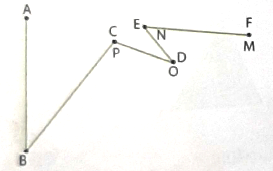
\includegraphics[width=1\linewidth]{6FMA108_imagens/imagem1}
			\begin{enumerate}[a)]
				\item (~~) O ponto $B$ é igual ao ponto $N$
				\item (~~) O ponto $A$ é diferente do ponto $M$.
				\item (~~) $O \neq D$.
				\item (~~) $F = M$.
				\item (~~) O segmento $\overline{BC}$ é igual ao segmento $\overline{CB}$.
				\item (~~) $\overline{AB} \cong \overline{EF}$
				\item (~~) $\overline{CD} = \overline{DP}$.
				\item (~~) O ângulo $B\hat{C}D$ é congruente ao ângulo $M\hat{N}O$.
				\item (~~) $C\hat{D}E \cong N\hat{O}P.$
			\end{enumerate}
			\item Com o auxílio de uma régua, responda se os triângulos a seguir são congruentes. Justifique. \\
			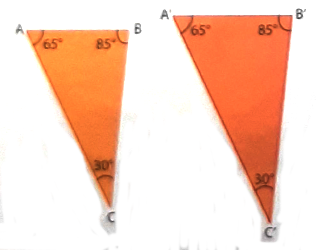
\includegraphics[width=1\linewidth]{6FMA108_imagens/imagem2}
			\\\\\\\\\\\\\\
			\item Observe as figuras a seguir. \\
			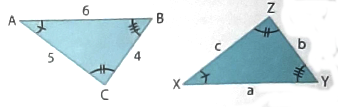
\includegraphics[width=1\linewidth]{6FMA108_imagens/imagem3}
			Sabendo que $\Delta$$ABC \cong \Delta$$XYZ$, calcule $a, b$ e $c$.
			\\\\\\\\\\\\\\
			\item Observe as figuras a seguir.
			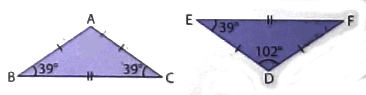
\includegraphics[width=1\linewidth]{6FMA108_imagens/imagem4}
			Os triângulos $ABC$ e $DEF$ são congruentes? Justifique sua resposta.
			\\\\\\\\\\\\\\
			%77 a 80
			\item Assinale \textbf{V} (verdadeiro) ou \textbf{F} (falso) para cada sentença. Justifique sua resposta.
			\begin{enumerate}[a)]
				\item (~~) Em um retângulo $ABCD, \overline{AB} \cong \overline{CD}$ e $\overline{AD} \cong \overline{BC}$.
				\item (~~) Os quatro lados de um quadrado são congruentes.
				\item (~~) Em qualquer retângulo $ABCD$, $\hat{AB} \cong \hat{AD}$.
			\end{enumerate}
			\item Os triângulos a seguir são congruentes? Justifique. \\
			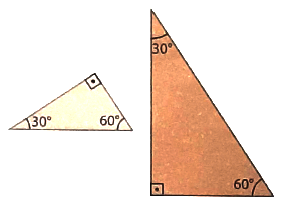
\includegraphics[width=1\linewidth]{6FMA108_imagens/imagem5} \\\\\\
			\item Os lados de um triângulo $ABC$ medem 9 cm, 12 cm e 15 cm. Sabendo-se que o $\Delta$$EFG$ é congruente ao $\Delta$$ABC$, calcule o perímetro do $\Delta$$EFG$. 
			\\\\\\\\\\\\\\\\\\\\\\\\
			\item Os triângulos $PQR$ e $TUS$ das figuras a seguir são congruentes. Calcule as medidas dos ângulos $P\hat{Q}R$ e $T\hat{S}U$ e determine o valor de $a + b$ \\
			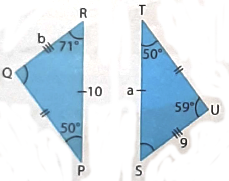
\includegraphics[width=1\linewidth]{6FMA108_imagens/imagem6}
		\end{enumerate}
		$~$ \\ 	$~$ \\ 	$~$ \\ 	$~$ \\ 	$~$ \\ 	$~$ \\ 	$~$ \\ 	$~$ \\ 	$~$
	\end{multicols}
\end{document}